\documentclass[letterpaper,twocolumn,10pt]{article}
\usepackage{usenix,endnotes,multirow}
\usepackage{refstyle,amsmath,chngcntr}
\usepackage{epsfig,subfigure,framed}

% Used for code snippets
\usepackage{listings,courier}

% Used for changing the spacing after the title, sections, and subsections.
\usepackage{titlesec,titling}

% Make text in figure captions small
\usepackage{caption3} % load caption package kernel first
\DeclareCaptionOption{parskip}[]{} % disable "parskip" caption option
\usepackage[small]{caption}

% Make sure that figure numbers are continuous through the document
\counterwithout{figure}{section}
\counterwithout{figure}{subsection}

% Settings on code listings.
\lstset{language=C,
		xleftmargin=0pt,
		xrightmargin=0pt,
		framexbottommargin=0pt,
        framextopmargin=0pt,
        framesep=0pt}

% Modify spacing before/after title, sections, and subsections.
\setlength{\droptitle}{-3em} 
\posttitle{\par\end{center}\vspace{-1em}}
\titlespacing\section{0pt}{12pt plus 4pt minus 2pt}{3pt plus 2pt minus 2pt}        
\titlespacing\subsection{0pt}{12pt plus 4pt minus 2pt}{3pt plus 2pt minus 2pt}   

% Compressed enumerations
\newenvironment{enumerate*}%
  {\begin{enumerate}%
    \setlength{\itemsep}{2pt}%
    \setlength{\parskip}{0pt}}%
  {\end{enumerate}}

% Compressed bibliograpgy
\let\ORIGbibliography\bibliography
\renewcommand{\bibliography}[1]{{\footnotesize \ORIGbibliography{#1}}}

% Add a horizontal rule above captions, and make captions closer to their figures
\DeclareCaptionFormat{ruled_caption}{\hrulefill\\#1#2#3}
\captionsetup[figure]{format=ruled_caption}
\let\ORIGcaption\caption
\renewcommand{\caption}[2][\compressedcaption]{%
\def\compressedcaption{#2}%
    \vspace{-12pt}%
    \ORIGcaption[#1]{#2}}

% Decrease spacing before \paragraphs
\titlespacing{\paragraph}{%
  0pt}{%              left margin
  0.5\baselineskip}{% space before (vertical)
  1em}%               space after (horizontal)


% Prevent footnotes from spanning multiple pages
\interfootnotelinepenalty=10000

% For leaving some comments in the draft.
\newcommand{\comment}[1]{}

\begin{document}

%don't want date printed
\date{}

%make title bold and 14 pt font (Latex default is non-bold, 16 pt)
\title{\Large \bf Debugging Kernel Modules with Behavioural Watchpoints}

%for single author (just remove % characters)
\author{
{\rm Peter Goodman} \hspace{1.5em} {\rm Akshay Kumar} \hspace{1.5em} {\rm Angela Demke Brown} \hspace{1.5em} {\rm Ashvin Goel}\\
University of Toronto
} % end author


\maketitle
\subsection*{Abstract}

Detecting bugs in large systems is challenging. TODO TODO TODO

In this paper, we outline our implementation of \emph{behavioural watchpoints}: a new mechanism for implementing program analysis and debugging tools. We describe three simple applications of our mechanism: detecting buffer overflows, detecting use-after-free and read-before-write bugs, and enforcing fine-grained memory access policies. 

In summary, we conclude.

%Finally, we present a brief case study on how we use behavioural watchpoints to detect misuses of the classical Read-Copy-Update (RCU) API in the Linux kernel.

%\iffalse
%	Some ideas for motivations:
%	\begin{enumerate}
%		\item Existing approaches to debugging are symptom based.
%		\item \texttt{gdb}-style breakpoints and watchpoints are tedious to use for detecting memory errors, and aren't helpful for detecting complex API misuses.
%		\item \texttt{printf}-style debugging is tedious because it requires annotating source code with print statements. This method of debugging generally ends up working, but it means inspecting logs, etc.
%		\item 
%	\end{enumerate}
%\fi

\section{Introduction}

A data \emph{watchpoint} is a powerful tool that reports on the usage of a particular memory location by a running program. Watchpoints are an integral feature of program analysis and debugging tools because they correlate watched memory locations with the program points accessing those memory locations. There are two categories of watchpoints: hardware-based and software-based. Hardware-based watchpoints are fast but scarce, which limits their usefulness as a means of perfoming large-scale program analyses \cite{UnlimitedWatchpoints}. Software-based implementations can scale to support millions of watchpoints \cite{DynamoRIOWatchpoints}, but are limited by their view of memory as an opaque sequence of bytes. This view is at odds with program analysis tools, which require contextual information about a program's memory. It is telling that watchpoint-based analysis tools must maintain separate bookkeeping mechanisms to recover contextual information about watched memory.

%However, complex program analysis tools require contextual information about a program's memory. It is telling that such tools must maintain separate bookkeeping mechanisms to recover this contextual information from their watchpoints.
%It is telling that software-based watchpoints are unsatisfactory for program analysis tools because these tools 
% tools because these tools must employ separate bookkeeping mechanisms that associate contextual information with watched memory.
%Implementing complex program analyses requires contextual information about watched memory, which must be separately maintained. 
%This extra bookkeeping
%acceptable for program analysis, but are limited by their all-or-nothing, shadow-memory-based approach. Program analysis tools that require contextual information about watched memory must implement new shadow memory schemes.
% needed by analysis tools requires different shadow memory schemes.
%Software-based watchpoints are acceptable for program analysis, but current implementations employ an all-or-nothing, shadow-memory-based approach to provide contextual information about watched memory.
% use of shadow memory to provide contextual information 
%fail to provide contextual information about watched memory.
%; however, they fail to 
%Software watchpoints typically come in two forms: coarse- and fine-grained. Coarse-grained watchpoints 
%Existing implementations of software watchpoints 
%accesses to particular memory locations with the program locations making those accesses. 
%Watchpoints are an integral feature of program analysis and debugging tools as they highlight the location where some memory of interest is used.
%Existing program analysis and debugging tools make heavy use of watchpoints 

%In this paper, we address the scalability concerns of hardware-based watchpoints and the incongruency between the implementation and usage of software-based watchpoints for program analysis.


%introduce \emph{behavioural watchpoints}: a new form of software-based watchpoints that simplify the implementation of program analysis and debugging tools. 
% \comment{Behavioural watchpoints are an easy-to-use mechanism that simplify the implementation of debugging and analysis tools.}

In this paper, we introduce \emph{behavioural watchpoints}: a new form of software-based watchpoints that simplify the implementation of program analysis and debugging tools.  Behavioural watchpoints address the scalability concerns of hardware-based watchpoints and overcome the incongruency between how software implements watchpoints and how program analysis tools use watchpoints.

%implementation and usage of traditional software-based watchpoints by program analysis tools.

Two characteristics define behavioural watchpoints:
\begin{enumerate*}
	\item[i)] Context-specific information is embedded in each watchpoint. This information is directly available when a watched address is accessed.
	\item[ii)] The action taken when a watched address is accessed is a component of the context-specific information. This implies that different watchpoints can \emph{behave} differently.
\end{enumerate*}

%What does it mean to be behavioural?
%What it means is that context-specific information is embedded in each watchpoint, and the action invoked when a watched address is accessed is a component of the context-specific information.

%Behavioural watchpoints are behavioural insofar as the actions invoked when watched memory is accessed is included 
% action performed when watched memory is accessed is contex

%they combine contextual information about watched memory with actions (i.e. behaviours) that are invoked when that memory is accessed.

%are \emph{behavioural} insofar as they tie together actions (\emph{behaviours}) to perform with  contextual information when watched memory is accessed.


%A \emph{behaviour} is a programmer-specified callback function that is invoked when memory is accessed (in)directly through a watched address.
\noindent
Behavioural watchpoints have several novel features:
\begin{enumerate*}
	\item[i)] {\bf Unrestricted:} A single watchpoint watches many addresses. In \Secref{buffer_overflows}, we use this feature to detect various kinds of buffer overflows.
	\item[ii)] {\bf Extensible:} Watchpoints are easily extended by programmers. In \Secref{uninitialised_memory}, we use this feature to implement selective memory shadowing and detect reads from uninitialised memory.
	\item[iii)] {\bf Type-specific:} When a watchpoint is added to an address, the address's type determines which set of behaviours to invoke when (displacements of) that address are dereferenced. In \Secref{access_policies}, we use this feature to detect Linux kernel rootkits by implementing fine-grained memory access policies.
%	\item[iv)] {\bf Easy-to-use:} TODO TODO TODO
%as a means of tracking and providing more robust information to watchpoint behaviours.
\end{enumerate*}


%address the asymmetry between how software-based watchpoints are implemented and how they are used by program analysis tools. In the process, we introduce a powerful new framework

%. A hardware watchpoint triggers an exception when its watched address is derefenced.
%A hardware watchpoint triggers an exception when a watched address is dereferenced.
%for debugging and analysing uses of memory in a running program. 



%The insight of our paper is that watchpoints provide a powerful framework for simplifying the implementation of program analysis and debugging tools.
%In this paper, we introduce behavioural watchpoints as a powerful framework that addresses the challenges of implementing DBT-based program analysis tools.
%we introduce behavioural watchpoints: a powerful framework for simplifying the implementation of DBT-based program analysis tools.

%is not widely adopted by the broader community 


%While many useful DBT-based program analysis tools exist, implementing these tools typically requires expert knowledge of low-level processor architecture details.

%While useful, implementing non-trivial analysis tools with existing binary translation toolkits \cite{DynamoRIOKernel,DynamoRIO,PinOS} is challenging. Most examples 

%Mostly people show simple uses of these toolkits and their performance, but they are not used widely because of the complexity of programming with them. The insight is that watchpoints provide a powerful framework for simplifying the implementation of various types of debugging and analysis tools. Hardware watchpoints are too limited and hence used sparingly. why. an infinite number of software watchpoints is a great idea, but still hard to use. why. that motivates "behavioral" watchpoints, and how they allow all kinds of cool potential applications.


% particularly when low-level architecture details are exposed.


%TODO TODO TODO
%A watched address is a memory address that encodes meta-information in its high-order bits. This meta-infomration distinguishes watched addresses from unwatched addresses, and is used by our run-time system to locate and invoke watchpoint-specific behaviours. 


%The embedding of meta-information is such that any (typical) displacement of a watched address is also a watched address, and shares the same meta-information.


%A behvaioural watchpoint is a tool that invokes a callback function (called a \texttt{behaviour}) to all reads and writes within an arbitrary range of memory addresses.
%\emph{behaviour} to the accesses of 
%instrumentation of  
%Behavioural watchpoints are a mechanism for instrumenting accesses to the memory of an object. 
%Unlike a normal memory address, a watched address encodes meta-information that in its high-order bits. The run-time system uses this meta-information to distinguish between watched and unwatched addresses. If an address is watched, then the run-time 
% locate 

\section{Implementation}
We implemented behavioural watchpoints using Granary: an extension of the DynamoRIO Kernel dynamic binary translation (DBT) framework \cite{DynamoRIOKernel,GranaryAtOSDI}. DBT is a useful technique for implementing dynamic program analysis and debugging tools \cite{Memcheck,DynamoRIOWatchpoints}. A dynamic binary translator is a program that rewrites the binary instructions of a ``guest" program while the guest program executes.

Granary was the DBT framework of choice for two reasons: 
\begin{enumerate*}
	\item[i)] Our goal was to analyse Linux kernel modules. Granary permits fine-grained instrumentation of the instructions of a running Linux kernel module.
	\item[ii)] Granary exposes rich type information about the Linux kernel. Granary has the ability to substitute the execution of a known function with a \emph{wrapped} version of itself. A wrapped function has the same type specification as its unwrapped counterpart and can freely modify its arguments and return value. This feature of Granary exposes type information which is used by behavioural watchpoints.
	%This information is a necessary component for making watchpoints ``behavioural".
\end{enumerate*}


%Granary permits fine-grained translation and instrumentation of the instructions of a running Linux kernel module. 


%\subsection{Design}

%Although there are many DBT toolkits \cite{DynamoRIOKernel,DynamoRIO,PinOS}, DBT as a technique has not seen widespread adoption.  DBT toolkits are challenging to use because they operate at a low level: binary instructions. By necessity, behavioural watchpoints require low-level access to perform fine-grained memory instrumentation. The novelty of watchpoints is their interface, which enables high-level, context-specific reasoning about low-level memory accesses.


%This characteristic of DBT enabled the implementation of behavioural watchpoints, which perform low-level memory instrumentation. However, by design, behavioural watchpoints provide a high-level interface, which 

%Although there are many binary translation toolkits \cite{DynamoRIOKernel,DynamoRIO,PinOS}, DBT as a technique has not seen widespread adoption because of the challenges involved in implementing non-trivial analysis tools.

%Behavioural watchpoints solve this problem by enabling low-level memory instrumentation 

%Despite these challenges, the flexibility of DBT enabled the creation of behavioural watchpoints.

% motivated the creation of a mechanism to simplify the development of program analysis tools: behavioural watchpoints.


%This aspect of existing DBT tools was a motivation for making behavioural watchpoints accessible and easy-to-use.

%


\subsection{Architecture}

\begin{figure}
\begin{center}
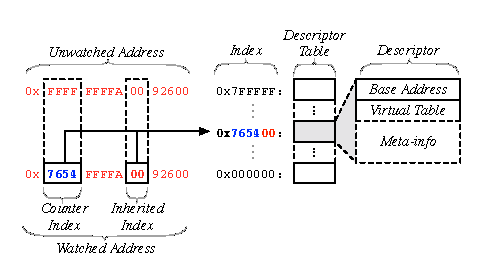
\epsfig{file=watchpoints.eps}
\end{center}
\caption{\label{fig:watchpoint_descriptor_table}A watched address and its corresponding unwatched address are compared. The process for allocating and resolving the watchpoint descriptor for the watched address is shown.}
%A 64-bit unwatched address is translated into a watched address.The index into the watchpoint descriptor table is composed of 23 bits from the watched address. This index is created by concatenating bits $[20,27]$ from the unwatched address with the next available partial index counter. This counter is located in the partial index counter table at the index represented by bits $[20,27]$ from the unwatched address.
\end{figure}

The implementation of behavioural watchpoints distinguishes between watched addresses and their descriptors.

A \emph{watched address} is a pointer with an index into the \emph{watchpoint descriptor table} embedded in its bits (\Figref{watchpoint_descriptor_table}). The $23$-bit index into the descriptor table is formed by concatenating bits $[20,27]$ (called the \emph{counter index}) with bits $[48,62]$ (called the \emph{partial index}). A watched address and its unwatched counterpart share the same counter index; however, the partial index of a watched address varies\footnote{This feature of watchpoints allows for a one-to-one mapping between a watched and unwatched address, and a one-to-many mapping between a watchpoint and all addresses watched by that watchpoint. The one-to-one mapping is formed by masking the high-order bits containing the partial index.}. Partial indexes are recorded in the \emph{partial index counter table}. When a watchpoint is allocated, the current value stored in the counter table for that specific counter index is incremented and returned as the watchpoint's partial index. This allocation strategy allows for at most $2^{15}$ watchpoints per counter index or megabyte of memory\footnote{x86 has byte-addressable memory. The counter index begins at bit $20$, giving each watchpoint $1$ MB = $2^{20}$ B degrees of freedom. However, if an over/underflow across the 1 MB-aligned boundary occurs then the counter index will be corrupted. We can correct one bit of corruption by requiring that the counter index and the partial index have the same sign. An alternative solution is uses a different indexing scheme. We have successfully experimented with a different indexing scheme that solves the aforementioned overflow errors, but sacrifices the one-to-one relationship between a watched and unwatched address.}.


%For each counter index, there can be at most  partial indexes.

%and unwatched addresses share the same counter indexes, b

A \emph{watchpoint descriptor} is a data structure containing a base address, a pointer to a virtual table (vtable) of memory operations, and programmer-defined meta-information. Each vtable provides eight functions: four read and four write functions. Each function is specific to a memory operand size (1, 2, 4, or 8 bytes). A watchpoint is initialised with either a generic or a type-specific vtable pointer. Type-specific vtables are specific to the \emph{type} of the watched pointer. When invoked, a vtable function operates on the watched address and its descriptor. Behavioural watchpoints earn their name from their ability to behave differently based on the meta-information stored in the descriptor and the (type-specific) vtable function invoked.

%The extension of watchpoint descriptors with programmer-defined meta-information combine with vtable functions to 
%The combination of programmer-defined meta-information and type-specific vtables 
%Such vtables are used to great effect in our memory-related bug detection applications (\Secref{applications}).

A watchpoint is added to a previously unwatched pointer by adding an entry to the watchpoint descriptor table and embedding part of the index of the entry in the high-order bits of the pointer. The original value of the pointer is saved as the base address of the descriptor. A watchpoint is removed from a pointer by masking the high-order bits containing the partial descriptor index. This approach permits a one-to-one mapping between a watched address and its unwatched counterpart, while allowing a single descriptor to watch many addresses. Specifically, a single watchpoint can watch up to $2^{20}$ distinct addresses, and each megabyte of memory can be watched by up to $2^{16}$ distinct watchpoints.

%at most $2^{20}$ different addresses.

Watched addresses, however, do not reference valid memory. Dereferencing a watched address triggers a hardware exception. To avoid this, we use Granary to dynamically translate memory loads and stores to first check for and then resolve watched addresses to their unwatched counterparts. If a watched address is detected then a watchpoint-specific vtable function is invoked. Both the address of the watchpoint descriptor and the watched address are passed as arguments to the invoked function. Finally, the original memory instruction is emulated by one that uses the unwatched address. The choice of which vtable function to invoke depends on the size of the memory operand (1, 2, 4, or 8 bytes) and whether the operation reads or writes its operand from/to memory.

%Watchpoints are created by adding an entry to the watchpoint descriptor table, and modifying a pointer in-place to include 
%The structure of a watched address is such that any displacement of a watched address will associate with the original
%Watchpoints associate zero or more watched addresses with a single watchpoint descriptor, located in the . 
%\subsection{Optimizations}

\section{Applications\label{sec:applications}}
The following sub-sections describe three applications of behavioural watchpoints and their implementations. In these sub-sections, we use the term \emph{object} to describe any value with a named location in memory.

\subsection{Buffer Overflows \label{sec:buffer_overflows}}
A buffer overflow is a software bug where a program--in an attempt to write to some object's memory--actually writes to adjacent memory cells. Detecting buffer overflows is important because they are commonly used in remote code execution and privilege-escalation attacks against operating systems \cite{SecureProgramExecFlowTracking}. One method of detecting buffer overflows relies on the compiler to allocate ``poisoned" regions of memory around each object \cite{AddressSanitizer}. Accessing this memory is an error because poisoned memory (which is transparently added by the compiler) does not exist as a named program entity. Our approach is similar in that memory adjacent to a watched object is considered poisoned; however, we do not rely on compiler support, nor do we allocate or mark poisoned memory as such.

We employ three overflow detection policies: heap-based, type-based, and stack-based. \comment{For uniformity, the blind policy is a special case of the targeted policy.} All three policies depend on the same extension to the meta-information of watchpoint descriptors: a \emph{limit address}. Together, the base address (stored in the descriptor) and the limit address delineate an object's boundaries in memory \cite{BccFatPointers}.

\paragraph{Heap-based overflow detection \label{sec:heap_overflow}}
\begin{figure}
\begin{lstlisting}[language=C,basicstyle=\footnotesize\ttfamily]
FUNC_WRAPPER(__kmalloc, (size, flags), {
  void *addr = __kmalloc(size, flags);
  ADD_WATCHPOINT(addr, size);
  return addr;
})
\end{lstlisting}
\caption{\label{fig:kmalloc_wrapper}Definition of the \texttt{\_\_kmalloc} function wrapper in Granary. The above code expands into a function for wrapping the \texttt{\_\_kmalloc} kernel memory allocator. Calls to \texttt{\_\_kmalloc} are transparently substituted with calls to the generated wrapper. The wrapper invokes the original \texttt{\_\_kmalloc} function and returns a watched version of the allocated address.}
\end{figure}

The heap-based detection policy detects buffer overflow errors on all heap-allocated objects. We use Granary to substitute invocations of the kernel's memory allocators (e.g. \texttt{kmalloc}) with wrapped versions of the allocators (\Figref{kmalloc_wrapper}). A wrapped allocator invokes the original allocator but returns a watched version of the allocated address. The watched address returned has its descriptor initialised with the base address as the allocated address and with the limit address as the base address plus the requested allocation size. All buffer overflow detecting watchpoints are initialised with the same vtable pointer.

%\comment{TODO: move first sentence into implementation}
%To detect buffer overflows (including heap-based overflows), we use the same vtable of operations and watchpoint meta-information (limit address).
%The vtable used by buffer overflow detecting watchpoints makes use of the operand size-specific nature of vtable functions.

The vtable pointer used by all buffer overflow detecting watchpoints points to a table of memory operand size-specific functions. The operand size is necessary to detect dereferences of memory that overlap both the object and its adjacent memory, as illustrated in case \emph{(3)} of \Figref{detect_overflow}. The vtable function corresponding to the memory operand size is invoked when a watched address is dereferenced. Each vtable function is programmed to check the watched address against the base and limit addresses stored in watchpoint's descriptor (\Figref{detect_overflow}). If a buffer underflow or overflow is detected then the vtable function notifies the run-time system.

\begin{figure}
\abovedisplayskip=0pt
\belowdisplayskip=0pt
\begin{center}
	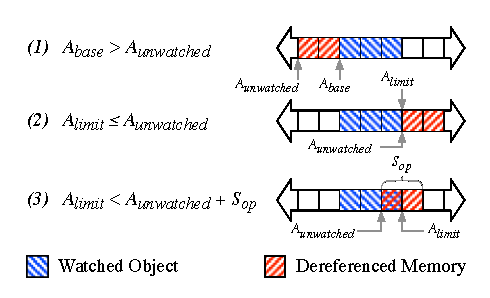
\epsfig{file=overflow.eps}
\end{center}
\iffalse
	\abovedisplayskip=0pt
	\belowdisplayskip=0pt
	\begin{align*}
		A_{base}  & > {A_{unwatched}} \tag{Underflow} \\
		A_{limit} & \leq {A_{unwatched}} \tag{Overflow} \\
		A_{limit} & < {A_{unwatched}} + S_{op} \tag{Overlap}
	\end{align*}
\fi
\caption[Caption for LOF]{\label{fig:detect_overflow}Three common buffer overflow cases are illustrated above: 1) underflow 2) overflow, and 3) overlap. Beside each illustration is the policy that detects the specific bug. When a watched address ($A_{watched}$) is dereferenced, a vtable function that is specific to the memory operand size ($S_{op}$) is invoked. This function detects a buffer overflow if the intended referenced memory address ($A_{unwatched}$) does not fall within the boundaries delineated by the base and the limit addresses ($A_{base}$ and $A_{limit}$, respectively).}
\end{figure}
%\protect\footnotemark
%\footnotetext{Policy (2) of \Figref{detect_overflow} is redundant but is illustrated for clarity.}

\paragraph{Type-based overflow detection}
The type-based detection policy is applied when the type of a pointer is known (i.e. not \texttt{void*}). The simplest use case of type information is to infer the limit address of a typed pointer. A more complex use case arises when the fields within a structure encode memory bounds information. In both cases, the vtable functions for typed and untyped memory operate in the same way.

%For example, a variable-sized array can be represented as a structure type with two fields: the number of objects in the array and a pointer to the array's objects. Out-of-bounds array accesses are detected by replacing the address of the array's objects in the structure with a watched address. The watchpoint's limit address is initialised to the address of the objects plus the number of objects in the array scaled by the size of each object. As before, the size of each object is inferred from the type of the object pointer field.

The type of an addressable object becomes known to Granary in the context of wrapped functions. Granary recursively follows argument and return value pointers based on object type specifications. These specifications tell Granary how to follow pointers and what--if any--pointers should be converted to watchpoints. To reduce programmer effort, Granary automatically generates type specifications and wrapper functions for any set of known types and functions. Some manual post-processing is required if the analysis/debugging application needs to understand semantic relationships between function arguments or structure fields. \comment{Automating this process was an important goal of Granary because of Granary wraps all (approx. 6,000) exported kernel functions.}

%If a pointer to that object is reachable from an argument to, or from the returned value of, a Granary-substituted wrapper function. Within a wrapper, Granary recursively follows argument pointers

%For example, if a function accepts a variable length array as an argument (encoded as a tuple of the size of the array and a pointer to the objects in the array) then a watchpoint can be used to detect out-of-bounds array accesses. Detecting such accesses requires replacing the address of the array's objects with the watched version of that address. The descriptor of this watchpoint is initialised with the number of objects in the array and the size of each object. Like the blind policy, the targeted detection policy performs the same addressability checks using the descriptor's meta-information.

\paragraph{Stack-based overflow detection}
Detecting stack overflows at the granularity of function activation frames requires more support from Granary's run-time system. At a high level, each activation frame is assigned a dedicated watchpoint when a function is called. The effect of an instruction that grows or shrinks an activation frame's size is reflected by a similar change to the base address\footnote{The run-time call stack on x86 grows into lower memory.\comment{ Modifying the base address instead of the limit address allows us to maintain one set of vtable functions for all three buffer overflow detection policies.}} of the frame's watchpoint descriptor. When a function returns, the descriptor of its activation frame is cleared, but remains allocated\footnote{Reclaiming/reusing allocated but unlikey-to-be-used watchpoints is challenging. One overflow-specific approach is to ensure that the next use of the watchpoint is for a buffer whose bounds do not intersect with the current use's bounds. Another approach is to use some number of context switches as a grace period in which the watchpoint cannot be reused, but after which it can be reused. We leave this as future work.} lest the address of a local variable escape the function\footnote{If the address of a stack-allocated object escapes its function activation frame, then that pointer is said to be \emph{dangling}. Dereferences of dangling pointers can cause stack overflow errors. In the kernel, data stored in unallocated stack memory (e.g. through a dangling pointer) is at risk of being clobbered by interrupt stack frames and by function activation frames.}.  

We assume that a memory instruction operating on a constant displacement of the stack or frame pointer registers is well-behaved. However, if the stack or frame pointer registers participate in a memory instruction and the displacement from the register is dynamically-bound then that instruction is suspect. An instruction that copies the address in the stack or frame pointer registers is also suspect because the copied address might escape the current function or participate in a local stack overflow. All suspect instructions are translated to transparently add the frame's dedicated watchpoint to the dereferenced or copied address.

%To prevent stack overflows on stack-allocated variables that escape the current function, we 
% is translated to use the current frame's watchpoint.
%An offsetted dereference of stack or frame pointer is suspect if the offset is dynamically bound. 
%We detect buffer overflows when the stack or frame pointers are derefe
%on dynamically offsetted dereferences of the stack or frame pointers, and aliases of the stack or frame pointers.
% Stack-based protection is extended to pointers that potentially escape the current function. For example, if an instruction copies the address stored in the stack or frame pointer registers into a third location, then that instruction is translated to add the frame's watchpoint to the copied address.

This scheme segments the runtime stack into contiguous but non-overlapping regions of watched memory. A straightforward extension excludes saved return addresses and link pointers from the known bounds of activation frames, thus detecting return-oriented buffer overflow attacks.

%The typical activation frame layout on x86 
%When a function is called, a watchpoint is allocated with its base and limit addresses to the address immediately below 
%Our approach uses watchpoints to segment the runtime call stack into its activation frames and is able to detect 
%a simple representation of a variable length array contains the size of the array and a pointer to the objects of the array. 
%counterparts are invoked. The type signature of the functions being wrapped betray 
%Each wrapped function can modify the (typed) arguments and return value 
%The type of a pointer is known to Granary when a function is invoke

%Granary uses a description of the layout a typed object to discover  pointers contained within the object, as well as relations between fields of an object.


%The structure of a referenced type betrays meaningful semantic information, which can. For example, a 
%Like the blind policy, the targeted detection policy uses the same meta-information to detect buffer overflows.
%This vtable is initialised with functions 
% The vtable pointer is initialised to point to a generic 
%The first policy uses Granary to wrap the Linux kernel memory allocation routines . The wrapped versions of these routines invoke their unwrapped counterparts, but modify their return values (the address of the newly allocated memory) by converting them to watchpoint addresses.


%Our approach depends heavily on Granary's ability to wrap known functions. 
% functionality to instrument 

%map to any semantically valid program references.
%erroneous program behaviour (buffer overflow) because poisoned regions of memory are transparently added by the compiler. 
%These poisoned regions, called red zones, trigger hardware exceptions when erroneously accessed.
%Adjacent memory cells can be ``poisoned" and accesses to poisened memory causes a hardware exception, 

\subsection{Uninitialised Memory Bugs\label{sec:uninitialised_memory}}

In this section, we show how to use behavioural watchpoints to detect uses of uninitialised memory.  Detecting such uses is important because a program using uninitialised memory can exhibit unintended, non-deterministic behaviour.

We define uninitialised memory as either allocated memory to which no value has been written, or de-allocated memory. We selectively track the initialisation state of each byte of watched memory using \emph{shadow memory} \cite{Memcheck}. Our implementation represents shadow memory as a bitset, where the state of each bit tracks the initialisation state of a byte of watched memory. Watchpoint descriptors are augmented to include the size (in bytes) of a watched object and a pointer to the memory shadowing the object\footnote{As an optimisation, shadow memory for small objects can be embedded in the watchpoint descriptor.}.

%As an optimisation, shadow memory for small objects (size $\leq$ 56 bytes) is embedded in the seven high-order bytes of the descriptor field containing the size of the watched object. For small objects, the shadow memory pointer points into the descriptor field storing the size of the shadowed object. Shadow memory is independently allocated for large objects. This optimisation does not prevent objects larger than $2^{8}$ bytes from being tracked: the descriptor's size field serves its dual role only when the object is small.

%This optimisation does not prevent objects. 
%For large objects, . Independent allocation of shadow memory for large objects implies
%do not interfere with this optimisation because the six high-order bytes only store 
%This optimisation assumes that no object is larger than . 
% In the kernel, the original address of shadow memory is recovered by masking the high-order bits. Shadow memory for small and large objects is accessed uniformly: the shadow memory pointer is masked before it is dereferenced. For small objects, the address of shadow memory is the address of the two high-order bytes of the descriptor field storing the pointer to shadow memory. For large objects, shadow memory is independently allocated.

We apply the above shadow memory scheme to detect uses of uninitialised memory for heap-allocated objects. As in \Secref{heap_overflow}, we interpose on the kernel's memory allocators and add watchpoints to the addresses returned by those allocators. When memory is allocated, the watchpoint descriptor is initialised with the number of allocated bytes (available as an argument to the allocator) and with its own shadow memory. The bits in shadow memory are initialised to zero.

\paragraph{Read-before-write bugs}
A read-before-write bug occurs when uninitialised memory is read by a program. This bug can cause non-deterministic behaviour because uninitialised memory can contain arbitrary values. If a control-flow instruction (such as a branch) decides its target based on the uninitialised value read from memory, then the resulting control-flow can be random.
 
%memory is read before it is written.
%Uninitialised memory bugs often go unnoticed, especially in complex code, 
%, by luck, the previous state of the read memory cells is
%This bug can cause non-deterministic behaviour 
%if the direction that a branch instruction takes is decided by the value stored in uninitialised memory.

%expects that reads of uninitialised memory 
%depends on there being a semantically meaningful value stored at the memory location being read.

All watchpoint descriptors for detecting uses of uninitialised memory are initialised with the same vtable pointer. The read-specific vtable functions report to the run-time system when the shadow bit corresponding to one of the read bytes is zero. The write specific vtable functions set to one all shadow bits that correspond to overwritten bytes. Both groups of vtable functions perform bounds checking\footnote{This check is functionally similar to \Figref{detect_overflow}, but uses the descriptor's base address and object size instead of using a base and limit address.} on the dereferenced address. 

Unlike our other memory error checking policies, the read-before-write bug policy detector can report false positives. It is common for larger-than-needed reads to be performed and for compiler-added structure padding to be read (but never written). A relaxed version of our read-before-write memory checking policy requires that at least one shadow bit is set for every read operation.

%The read-specific vtable functions look to see if any bit in the set of bits shadowing the bytes of memory being read is zero. A debugger breakpoint is triggered if a zero bit is found. The write-specific functions set the bits that shadow the bytes being overwritten to one.

\paragraph{Use-after-free bugs}
A use-after-free bug occurs when memory is accessed after it has been deallocated. This bug can cause non-deterministic behaviour if the once occupied memory of the  deallocated object is partially or fully reallocated for another purpose.

We use Granary to interpose on the kernel's deallocation functions (e.g. \texttt{kfree}). If the argument to a wrapped deallocator function is a watched address then the descriptor is cleared. Finally, the original deallocator is invoked with the unwatched address as an argument. Reads and writes to a watched address of a deallocated object fail to pass bounds checks because the object size is zero\footnote{Two positive side-effects of our approach is that it automatically detects double-free bugs and freeing of non-heap memory bugs. A double-free is detected when a watched address for an already deallocated object is passed as an argument to a deallocator. An attempt to free non-heap memory is detected when an unwatched address is passed as an argument to a deallocator.}.

%\footnote{When masked, the pointer to shadow memory for small objects points to itself. This enables uniform access to shadow memory for all object sizes.}.

%Watchpoint descriptors are augmented with a limit address and a dual-purpose 64-bit pointer to shadow memory. 

%Small objects ($\leq$ 16 bytes)

%The buffer overflow policies of \Secref{buffer_overflows} augments watchpoint descriptors with shadow memory

%An uninitialised memory bug is characterized as one where memory...

\subsection{Fine-grained Access Policies\label{sec:access_policies}}
In this section, we describe the implementation and use of the field-accessor API: a novel extension to behavioural watchpoints. We use this API to detect Linux kernel rootkits. Detecting rootkits is important because rootkits are malicious programs that infect and corrupt operating systems. Rootkits are difficult to detect because they have access to  privileged functionality, which allows them to hide their existence. However, rootkits often leave hints of their existence in the form of violated data structure invariants \cite{GibraltarKernelInvariants,OSck}. For example, \Figref{field_invariant_check} discusses an invariant which, if violated, can prevent an anti-virus program from scheduling periodic scans---scans which might otherwise detect the presence of a rootkit. We use the field-accessor API to actively detect violations of data structure invariants and report them to our run-time system as potential rootkits.

%We use the field-accessor API to actively detect violations of data structure invariants, thus 
%We detect rootkits by using the field-accessor API to detect violations of data structure invariants. 
%detects a violation of a data structure invariant that 
%We show how the field-accessor API enables Granary to detect violations
%kernel data structure invariants and
% and can easily hide themselves or prevent their own detection
%Detecting kernel rootkits is challenging because the entire surface area of an operating system kernel 
%We use the field-accessor API to detect Linux kernel rootkits. We detect rootkits by encoding data structure invariants 


The field-accessor API is a declarative API for interposing on memory reads and writes at the granularity of \texttt{C} structure (bit)fields. With the API, one can attach a callback function to memory reads/writes of a structure field (\Figref{field_invariant_check}). An attached read or write callback is invoked when the specific field within a watched object of the correct type is dereferenced. The type of an object is implicity resolved; watchpoint vtables are type-specific, and the field-accessor API is implemented in terms of watchpoint vtables. The code that connects vtables to attached callbacks is automatically generated. Generating this code involves parsing \texttt{C} header files and determining for each \texttt{C} structure type $T$, all fields accessed by a dereference within the memory occupied by a watched instance of $T$. If such a dereference occurs, then an attached callback function is invoked for each touched field.



%This extension is enabled by the type-specific nature of watchpoint vtables and by Granary's database of type information. We apply this extension to detect violations of data structure invariants in the Linux kernel. Detecting violations of kernel data structure invariants is important because such violations can signal the presence of kernel rootkits \cite{GibraltarKernelInvariants,OSck,LXFI}.

% The field-accessor API is an API for attaching a callback function to memory reads and/or writes of a structure field. 




%Because watchpoint vtables are type-specific, The type of the object is known to the watchpoint from the time at which it was added
%The type of the object is known from the point 
%Our extension is limited by its dependency on advance knowledge of the types used by an instrumented program. This limitation does not prevent us from checking invariants on arbitrary binary Linux kernel modules. 
%Detecting violations of data structure invariants is important as such violations can be a signal of buggy code or 
%Detecting such violations is important as they signal potential kernel rootkits .


%TODO TODO TODO: Properly introduce field-accesor API as an advanced use of the type-specific vtables.

%In this section, we describe the implementation and use of the field-accessor API: a novel extension to behavioural watchpoints. The field-accessor API permits interposing on memory reads and writes at the granularity of structure fields (including bitfields). We apply this API to detect violations of data structure invariants in the Linux kernel. Detecting violations of invariants can be used to detect kernel rootkits \cite{GibraltarKernelInvariants,OSck}.



%This requirement is not overly strict, as will be shown for Linux kernel modules.
%If a read or write callback is attached to a structure's field, and that field is accessed through a watched address, then its callback is invoked when that field is read from or written to memory.
% dereference of that field through a watchpoint
% defining per-structure-field read/write access callback functions. If a field in an object with a known structure type is dereferenced through a watched address, then its corresponding callback function is invoked. 

%The Linux kernel is a large software system with a complex and flexible API: exported functions, variables, and types. Extensions to the kernel, called modules, use this API to support new hardware (e.g. graphics drivers) and provide new features (e.g. file systems). However, misuses of data structures exposed through the API can lead to crashes or security breaches \cite{GibraltarKernelInvariants,OSck,LXFI}.

%The Linux kernel's exported API is defined across a set of \texttt{C} header files. We parse these files and automatically generate code that determines, for each type $T$, all fields ``touched" by a dereference within the memory occupied by a watched instance of $T$. If such a dereference occurs, then an attached callback function is invoked for each touched field.

\iffalse
	The steps taken to generate this code are described below:
	\begin{enumerate}
		\item Kernel header files are parsed. The set of all exported functions, variables, their dependent types, and the structure of those types is recorded.
		
		\item The recorded type information is transformed into a program that reports the bit boundaries of each structure field within its containing type. At runtime, this program creates zero-initialized instances of each type and selectively sets to one the bits of each of the type's internal fields. The bits of memory of each object are linearly scanned to determine the exact bounds of each field.
		
		\item The derived type layout information is processed to create a unique \texttt{C++} template class for each kernel structure type. A singleton instance of the instantiated template class for some type $T$ is the operations vtable for all watched objects of type $T$.
		
		The method bodies of the template class invoke attached field access callback functions. The choice of which callback(s) to invoke is statically determined for each possible dereference size (1, 2, 4, or 8 bytes) and byte offset into an object's memory. At runtime, the byte offset of a dereference of a watched object is computed by subtracting the descriptor's base address from the dereferenced address, modulo the size of the object's type.
			
		Our use of \texttt{C++} templates serves two purposes. First, if a watchpoint is never added to an object of type $T$, then the corresponding template is never instantiated. This reduces code bloat when Granary is compiled. Second, if a watchpoint is added to an object of type $T$, then template instantiation is what permits the correct and type-specific automatic initialisation of the vtable pointer in the watchpoint's descriptor.
	\end{enumerate} 
\fi

\Figref{field_invariant_check} shows how an invariant on the \texttt{ioctl} field of any watched object whose type is \texttt{struct file\_operations} is checked using the field-accessor API. 

\begin{figure}
\begin{lstlisting}[language=C,basicstyle=\footnotesize\ttfamily]
// Invariant: rtc_fops->ioctl == &rtc_ioctl
WATCH_WRITE(struct file_operations, ioctl, {
  if(&rtc_fops  == base_address
  && &rtc_ioctl != ioctl) {
    // potential attack: prevent an anti-
    // virus scan from being scheduled!
  }
})
\end{lstlisting}
\caption{\label{fig:field_invariant_check}This code example shows how to check invariant 1(h) from \cite{GibraltarKernelInvariants} using Granary's field-accessor API. The invariant checked prevents a (potential) kernel rootkit from installing its own \texttt{ioctl} handler into the Real-Time Clock. Anti-virus programs depend on this built-in \texttt{ioctl} handler to periodically schedule virus scans. Replacing this handler can prevent such scans from being scheduled, thus allowing the rootkit to go undetected.}
\end{figure}

% watched pointer of 


%it allows a programmer to define per-structure-field read/write access policies, which are invoked whenever a (third-party) binary module dereferences the fields of a watched pointer of the correct type.

%A caveat of our approach is that fine-grained 

%the type of objto be watched must be known in advance. However, 

%TODO: example of \texttt{get\_thread\_info}, to the task struct, to become a rootkit.
%Linux kernel modules interact with the kernel using a well-defined inteface: exported functions. Large amounts of sensitive data structures are shared over this interface, and the kernel expects that modules behave sanely.

%\section{Case Study: Detecting RCU Usage Bugs}
%We have established that behavioural watchpoints are useful for implementing memory error detection and protection policies. The extensibility of watchpoints, however, makes them useful for a broader range of applications. To that end, this section reports on some early results from our watchpoint-based tool that detects misuses of the classical Read-Copy-Update (RCU) API in the Linux kernel. Detecting misuses of the RCU API is important because RCU is increasingly (mis)used as the synchronization mechanism of choice within the Linux kernel \cite{RCUInLinux}.

%\subsection{Read-Copy-Update}
%RCU is a lock-free synchronization mechanism allowing reader and writer threads to operate concurrently on a shared data structure \cite{RCU}. RCU is applicable when the ratio of the number of reader to writer threads is high, and when reader threads can tolerate ``stale" data.

%RCU reader threads operate in a non-blocking manner and execute concurrently with writers. Because of this, some readers might observe stale data, e.g. reading the value of a pointer immediately before that pointer is modified by a writer. Writer threads serialize to prevent the coexistence of two divergent ``views" of a data structure. Serialization of writers in the Linux kernel is often implemented by having writer threads compete for a mutex or spinlock. It is typical for the winning thread to wait for all concurrently executing reader threads to complete their outstanding reads before making changes that might affect the consistency of the data structure. A reader thread announces the existence of outstanding reads to writer threads by grouping its reads of the data structure into a \emph{read-critical section}.

%\paragraph{RCU API}
%TODO

%\subsection{TODO}

\section{Evaluation}
TODO

\section{Conclusions and Future Work}
TODO

%The writer thread whose turn it is to modify the data structure waits for all concurrently executing reader threads to complete their outstanding reads of the data structure. Waiting ensures that reader threads do not observe inconsistent data.

%Reader threads signal the beginning and end of data structure reads by invoking \texttt{rcu\_read\_lock} and \texttt{rcu\_read\_unlock}, respectively.


%This characteristic of RCU naturally segments the liftetime of a data structure into \emph{generations}. Under this lens, the acquisition of mutual exclusion over a data structure by a writer thread is a signal that a generation is near its end. The true end of a generation occurs when the writer thread that acquired mutual exclusion waits for all reader threads to complete any outstanding reads of the data structure. When one generation ends, the next immediately begins. This implies the coexistence of multiple generations. Correct usage of the RCU API requires that 


%This view is complicated by the coexistence of multiple generations; however, correct usage of the RCU API ensures that an individual reader thread never ovserves 
%Multiple generations of a RCU-protected data structure may coexist; however, proper 
%is when all concurrently \emph{active} readers at the time 
%must acquire mutual exclusion over the entirety of a protected data structure before making changes that must be visible in the most up-to-date view of the data structure.
%RCU reader threads are permitted to read the protected data structure without 
%At a high level, RCU implicitly segments the lifetime of a data structure into \emph{generations}. As one generation ends, another automatically begins.
%A grace period
%A grace period ends delimited by a writer thread acquiring the exclusive right to modify values stored in the protected structure.
% over the entirety of the protected data structure.

%approach to synchronizing concurrently executing reader and writer threads. RCU is unique
%In this section, we describe an early implementation 


% The bibliography should be embedded for final submission.
\bibliographystyle{acm}
\bibliography{library}
\end{document}


